\section{weitere Bindungsarten, erlaubte Basenpaare}
 - Hoogsteen base pair\footnote{\url{https://en.wikipedia.org/wiki/Hoogsteen_base_pair}}\\
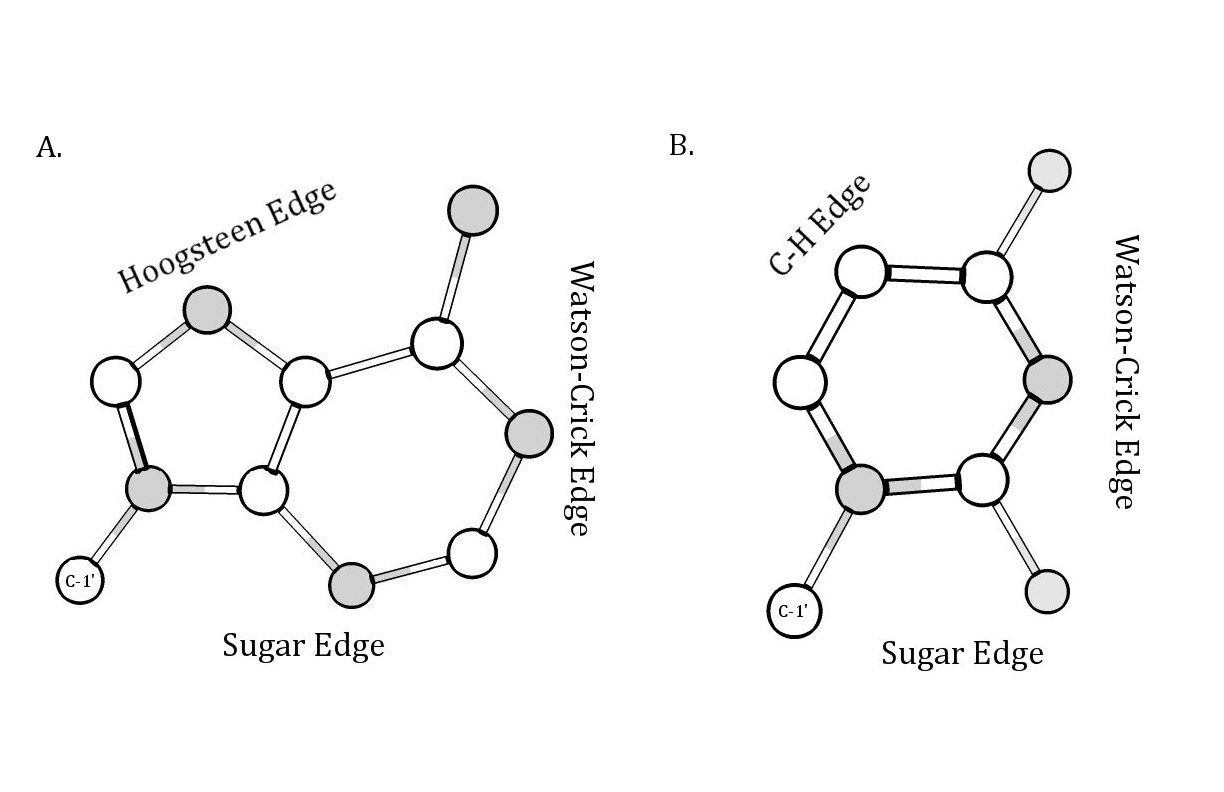
\includegraphics[width=0.5\textwidth]{lectures/160530/pix/Edge_Labels.jpg}
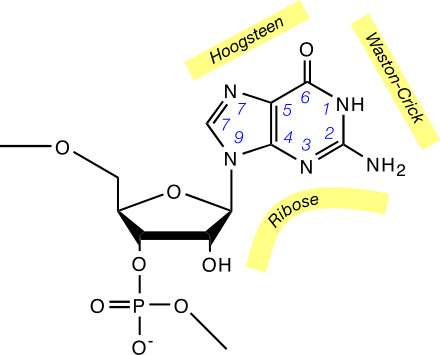
\includegraphics[width=0.5\textwidth]{lectures/160530/pix/440px-NucleotideFaces.jpg}

Jede Base kann mit jeder ihrer Kanten zu jeder Kante jeder Base ein Basenpaar bilden.
\\\\
\underline{Non-Standard Basepairs:}\\
Strukturmotive: Pattern von Standard basepairs führt zu speziellen 3D-Struktur (Kink-Turn)\\
Bifurcations (tripletts meistens)
12 * 12 * 2 mögliche Basenpaare: \textcolor{red}{Warum 288?}\\

Darstellung:\\
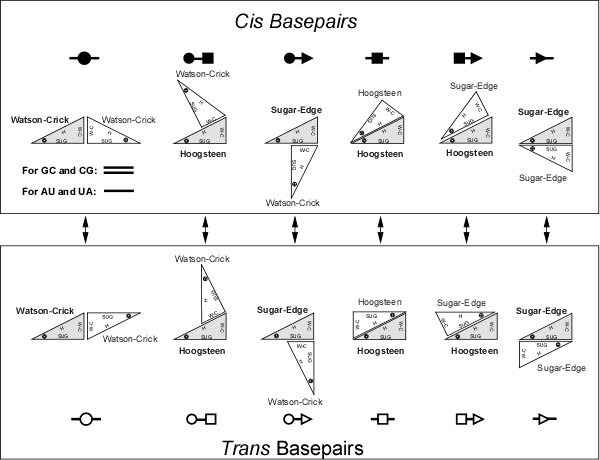
\includegraphics[width=0.85\textwidth]{lectures/160530/pix/geometric-family.jpg}
\\\\
\underline{Isoelektrische Basenpaare}\\
Änderung eines isoelektrischen Basenpaars gegen ein anderes ändert nichts an der Struktur\\
Listen von isoelektrischen Basenpaaren erstellt von Leontis und Westhof\\

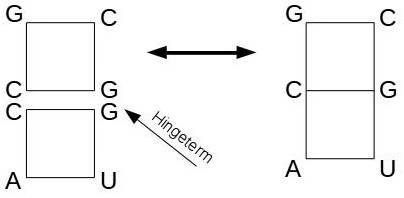
\includegraphics[width=0.5\textwidth]{lectures/160530/pix/hingeterm.jpg}
\\\\
Programme: MC-Fold, RNAWolf\\

\section{Proteine}

\begin{itemize}
	\item 20 Aminosäuren
	\item drei positiv geladene Aminosäuren (basisch): Arg (R), His (H), Lys (K)
	\item zwei negativ geladene Aminosäuren (sauer): Asp (D), Glutaminsäure (E)
	\item sehr unterschiedlich in den Seitenketten
	\item Verbindung durch Peptidbindung
\end{itemize}

Frage: Wie rotieren Aminosäuren, die durch eine Peptidbindung verbunden sind, im Räum?\\
Stichworte: Cis, Torsionswinkel\\

\underline{Ramachandran Plot:}\footnote{\url{https://en.wikipedia.org/wiki/Ramachandran_plot}}\\
allgemeines Beispiel:\\
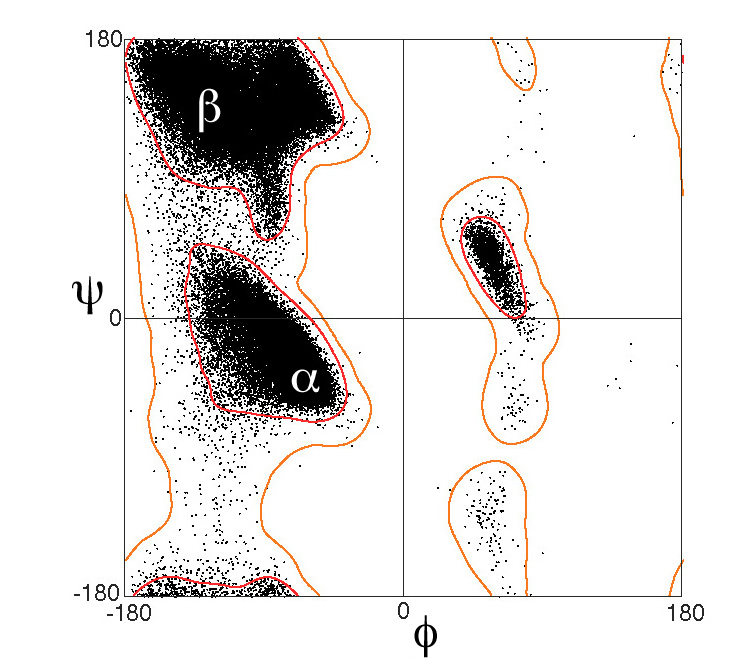
\includegraphics[width=0.3\textwidth]{lectures/160530/pix/Ramachandran_plot_general_100K.jpg}

\section{Sekundärstrukturelemente}
%https://de.wikipedia.org/wiki/Sekund%C3%A4rstruktur
 - Unterscheidung in drei Haupttypen\footnote{\url{https://de.wikipedia.org/wiki/Sekund\%C3\%A4rstruktur}}\\
\underline{Proteine:}
\begin{itemize}
	\item Helix $\alpha$-Helix (häufigstes)
	\begin{itemize}
		\item coiled-coli-Struktur: Helix umgeben mit einer Helix
		\item Transmembranhelices: 20 - 30 Aminosäuren, hydrophob, gehen durch die Zellmembran durch
	\end{itemize}
	\item Extended-Faltblatt: mindestens zwei Faltblätter immer zusammen, da dieses sich gegenseitig stabilisieren
	\begin{itemize}
		\item parallel, antiparallel
	\end{itemize}
	\item Turn (drehen der Backbonerichtung)
	\item Coil (Rest)
\end{itemize}

drei Helixe: Unterscheidung, was und wie viel zwischen den Wasserstoffbrückenbindungen steht\footnote{\url{https://en.wikipedia.org/wiki/Protein_secondary_structure}}
\begin{itemize}
	\item $\alpha-Helix$: 3,6,13-Helix (Helix zwischen 3. und 6. Atom, dazwischen liegen 13 Atome)
	\item $\pi-Helix$: 4,1,16
\end{itemize}

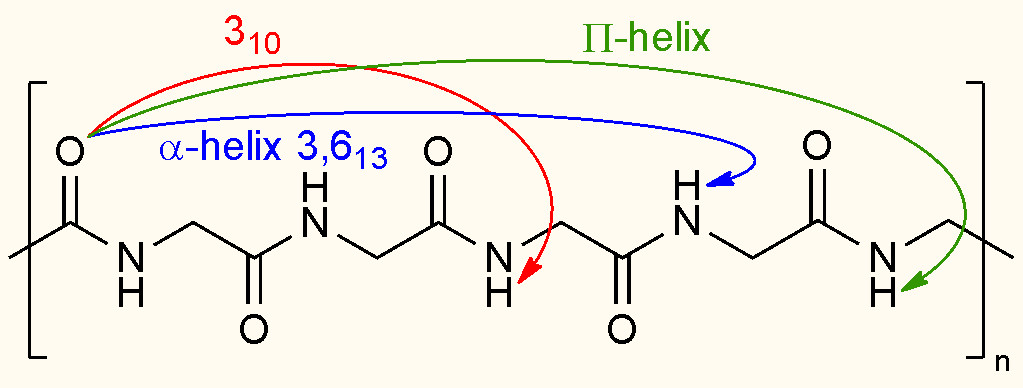
\includegraphics[width=1\textwidth]{lectures/160530/pix/Hydrogen_bridging_in_proteins.jpg}

\subsection{Chou-Fasman (Sekundärstrukturvorhersage von Proteinen)}
 - ca. 50\% Genauigkeit
\begin{itemize}
	\item 3 Tabellen mit Scores für $\alpha$ (Helix), $\beta$ (Faltblatt) und t (Turn) für alle Aminosäuren
	\begin{itemize}
		\item z.B. gut für Helix: Glu (1,51), Met Ala, Leu
		\item schlecht für Helix: Pro, Gly (0,57)
		\item gut für Faltblatt: Val (1,7), Ile (1,6)
		\item schlecht für Faltblatt: Asp, Glu (0,37), Pro (0,55)
	\end{itemize}
	\item Unabhängig voneinander $\alpha, \beta, t$ bewerten:
	\begin{itemize}
		\item nucleation: 4 von 6 Aminosäuren haben $S_{(\alpha)}$ > 1,03\\
		Erweitern nach links und rechts, bis Durchschnitt der letzten 4 AS $S_{(\alpha)}$ < 1 haben
		\item $\beta$: 3 von 5 Aminosäuren sollen $S_{(\beta)}$ > 1 haben, letzten 4AS $S_{(\beta)}$ < 1
	\end{itemize}
		\item Turn: $score(t)=S_{(t)}(x1) \cdot S_{(t)}(x2) \cdot S_{(t)}(x3) \cdot S_{(t)}(x4)$
\end{itemize}

\underline{Weiterentwicklung:}\\
 - nicht nur eine Aminosäure sondern gesamte Umgebung anschauen\\\\
\underline{GOR-Algorithmus:}\footnote{\url{https://en.wikipedia.org/wiki/GOR_method}}\\

 - bis zu 70\% genau
 - es gibt GOR1 bis GOR5, unterschiedliche Berechnungen
\begin{itemize}
	\item drei Matritzen mit Scores\\
	20 x 17 Matritze ($\alpha, \beta, turn$)\\
	Beispiel für $\alpha$: waagerecht: -8 bis +8, senkrecht alle Aminosäuren
	\item Score aus Summierung über Matrixeinträge, dann ähnliche wie Chou-Fasman
\end{itemize}

Beispiel: ACCTYRAR\underline{R}GHSTFYSW\\
für R
$S_{\alpha}=S^{\alpha}(-8,A) + S^{\alpha}(-7,C) + ... + S^{\alpha}(8,W)$\\
 - das für alle Sekundärstrukturelemente
\\\\
\underline{weiterer Algorithmus: SPIDER2}
\begin{itemize}
	\item ca. 80\% genau
	\item Winkel zwischen Aminosäuren berechnen
	\item Surface Accesible Area
	\item Sekundärstrukturen
\end{itemize}

Physikalische Eigenschaften von Aminosäuren:\\
\begin{itemize}
	\item sterischer Parameter (graph shape index: dünnes oder dickes Molekül)
	\item Hydrophobizität
	\item Polarisierbarkeit
	\item Isoelektrischen Punkt
	\item Helix Wahrscheinlichkeit
	\item Volumen
	\item Falblattwahrscheinlichkeit
	\item zusätzlich mit psi-Blast: PSSM ermitteln (kein Ergebnis für Struktur sondern nur für Sequenz!)
\end{itemize}

dann alle diese Parameter in neuronales Netz stecken:\\
% Bild 4 einfügen neuro_net.jpg
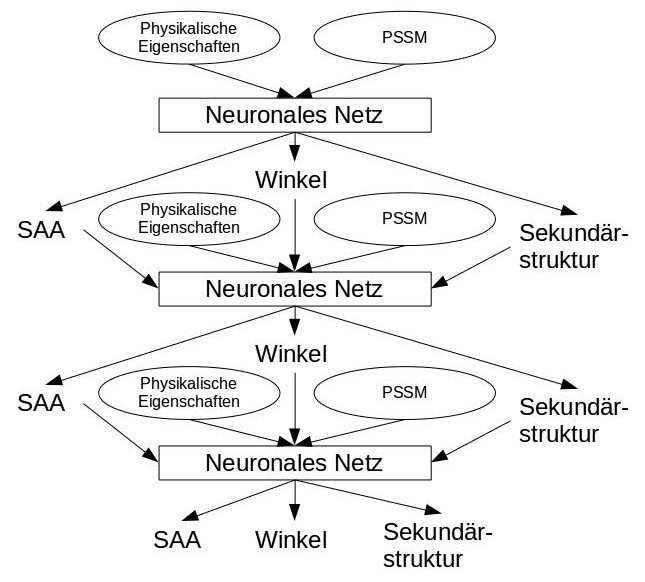
\includegraphics[width=0.7\textwidth]{lectures/160530/pix/neuro_net.jpg}
\\\\
w\textbf{eitere Möglichkeit: Meta Server}\\
\begin{itemize}
	\item ruft mehrere Algorithmen auf
	\item höhere Wahrscheinlickeit durch vergleichen der Ergebnisse (z.B. majority vote)
\end{itemize}